% ===================================================================================================
%                                                 |                                                 |
%                                                 |                                                 |
% -------------------------------------------- SECTION ---------------------------------------------|
%                                                 |                                                 |
%                                                 |                                                 |
% ===================================================================================================
\section{Learning paradigms for embodied AI (EAI) agents}\label{sec:learning_paradigms}
In this section we model the scaling of energy and time demand that results from the use of a team of robots learning a universe $\mathcal{S}=\left\lbrace s_1,s_2,\ldots s_j,\ldots, s_{N_\mathcal{S}}\right\rbrace$ of skills, with $|\mathcal{S}| = N_\mathcal{S}$.

% ===================================================================================================
\subsection{Energy and time demand for learning skills}
%---
\begin{tcolorbox}
	\begin{definition}\label{definition:complexity}
		The complexity $c_j$ of a skill $ s_j $  is the number of trial episodes $n$ needed to successfully learn the skill; i.e., all actions and states visited until a stopping criterion is reached. 
	\end{definition}
\end{tcolorbox}
% ---

%To simplify the analysis we make the conservative assumption that the power $P_0$ required by any given robot to learn of a skill is constant. Furthermore,% ---
To simplify the analysis consider the following conservative assumption
% ---
\begin{tcolorbox}
	\begin{assumption}\label{assumption:time}
		Given a large number of robots performing a large number of skills, the average power $P_0$ required by any given robot during learning and the average time $\Delta t$ allocated to the execution of every trial episode $n$ are constant, see Fig.~\ref{fig:power_per_episode}.
	\end{assumption}
\end{tcolorbox}
% ---
% ---------------------------------------------------------------------------------------------------
\subsubsection{\textbf{Episode, skill, and skill set energy requirements}}
% ---
\begin{figure}[!t]
	\centering
	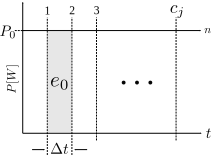
\includegraphics[width=0.95\columnwidth]{fig/power_per_episode.png}
	\caption{Power consumption per episode.}
	\label{fig:power_per_episode}
\end{figure}
% ---
Under Asm.~\ref{assumption:time}, the energy consumption of the $n$-th episode $e_j(n)$ is the constant product
% ---
\begin{equation}\label{eq:energy_per_episode}
    e_j(n) = \underbrace{P_0 \Delta t}_{\text{constant}} = e_0.
\end{equation}
% ---
Consequently, the energy consumed by a robot learning a skill $ s_j $ is directly proportional to the skill complexity $c_j$; i.e.
% ---
\begin{equation}\label{eq:energy_per_skill}
    E_j =\sum_{n=1}^{c_j} e_j(n) = e_0c_j.
\end{equation}
% ---
The energy spent on learning $\mathcal{S}$ under the absence of knowledge transfer is
% ---
\begin{equation}\label{eq:total_energy}
	E_{\mathcal{S}} = \sum_{j=1}^{{N_{\mathcal{S}}}} E_j = e_0 \sum_{j=1}^{{N_{\mathcal{S}}}} c_j%N_{\mathcal{T}} \cdot e_0 \cdot c_j 
\end{equation}
% ---
% ---------------------------------------------------------------------------------------------------
\subsubsection{\textbf{Time requirement}}
Similarly, the total learning time $T_{\mathcal{S}}$ for a simple agent is
% ---
\begin{equation}\label{eq:total_energy}
	T_{\mathcal{S}} = \Delta t \sum_{j=1}^{{N_{\mathcal{S}}}} c_j.
\end{equation}
% ---
As a consequence of Asm.~\ref{assumption:time} and \eqref{eq:energy_per_skill}, in the remaining of this section analyzing the complexity of a skill or set of skills is equivalent to analyzing the energy demand of its learning process.
% ===================================================================================================

\subsection{Similarity and knowledge}
%---
\begin{tcolorbox}
	\begin{assumption}\label{assumption:skill_clustering} If the similarity among a set of skills is significant, the exchange of acquired knowledge from these skills expedites the overall learning process.
		\end{assumption}
\end{tcolorbox}
% ---
Let $\mathcal{Z}_k \subset \mathcal{S}$ be a subset of $N_{\mathcal{Z}_k}$ skills that share high similarity; i.e. a \emph{cluster} of similar skills, see Fig.~\ref{fig:skill_similarity}. Furthermore, consider a second set $\mathcal{\zeta}_k \subset \mathcal{Z}_k$ that denotes already learned skills from $\mathcal{Z}_k$. Asm.~\ref{assumption:skill_clustering} implies that the $j$-th skill in the $k$-th cluster $s_{j,k} \in \mathcal{Z}_k$ can always benefit from the knowledge contained in $\mathcal{\zeta}_k$. This implies that the more skills enter $\mathcal{\zeta}_k$, the less knowledge about $ s_{j,k} $ will remain to be learned.
% ---
\begin{figure}[!t]
	\centering
	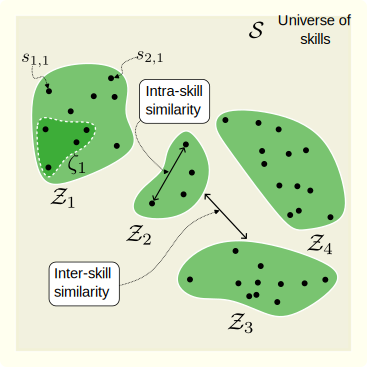
\includegraphics[width=0.95\columnwidth]{fig/skill_similarity.png}
	\caption{Similar skills in $\mathcal{S}$ can be grouped into clusters $\mathcal{Z}_k$.}
	\label{fig:skill_similarity}
\end{figure}
% ---
Now, we introduce a function $\bar{\sigma}_{j,k}\left(n\right)\in [0,1]$ that expresses the knowledge about a skill $s_{j,k} \in \mathcal{Z}_k\textbackslash \mathcal{\zeta}_k$ that \textbf{is not} contained in $\mathcal{\zeta}_k$. The function $\bar{\sigma}_{j,k}(\cdot)$ satisfies:
% ---
%\begin{itemize}
%	\item $\bar{\sigma}_{j,k}\left(n\right) = 1$, if $\mathcal{\zeta}_k=\emptyset$ or if it does not contain knowledge about the skill $s_{j,k}$
%	\item $\bar{\sigma}_{j,k}\left(n\right) = 0$, if \emph{all} the knowledge about skill $s_{j,k}$ is contained in $\mathcal{\zeta}_k$
%\end{itemize} 
% ---
\begin{equation}\label{eq:sigma_bar_conditions}
	\bar{\sigma}_{j,k}\left(n\right) = 
	\begin{cases}
		1 & \text{$\mathcal{\zeta}_k=\emptyset$}\\
		0 &\text{$\mathcal{\zeta}_k$ has \emph{all} knowledge of $s_{j,k}$}
	\end{cases}
\end{equation}
Conceptually, $\bar{\sigma}_ {j,k}\left(\cdot\right)$ is the fraction of knowledge from ${\mathcal{Z}_k}$ that remains to be learned.

% ---------------------------------------------------------------------------------------------------
\subsubsection{\textbf{Leveraging the acquired knowledge}}
To evaluate the effect of knowledge exchange during learning we introduce an upper bound called the skill \textit{fundamental complexity}.
% ---
\begin{tcolorbox}
	\begin{definition}\label{assumption:fundamental_complexity}
		The fundamental complexity $c_0$ describes the maximum number of trial episodes required to learn \emph{any} skill.
	\end{definition}
\end{tcolorbox}
% ---
If, in learning a skill $ s_{j,k} $, a robot uses the knowledge contained in $\mathcal{\zeta}_k$; then, two effects take place:
% ---
\begin{enumerate}
	\item There is less remaining knowledge, reflected in the initial value; i.e. $\bar{\sigma}_{j,k}(0) < 1$
	\item The knowledge acquisition rate increases
\end{enumerate}
% ---
%associated complexity $ c_{j,k} $ is necessarily smaller than the fundamental complexity $c_{0}$; i.e. $c_{j,k} < c_0~\forall j>1$.
This implies that the remaining knowledge scales down as a function of the number of learned skills $N_{\zeta_k}=|\mathcal{\zeta}_k|$. As a consequence, the complexity $c_{j,k}$ of said skill is smaller than the fundamental complexity $c_0$.%, as exemplified in Fig.~\ref{fig:complexity_per_cardinality}. 

The effects of knowledge exchange lead us to introduce another assumption.
% ---
\begin{tcolorbox}
	\begin{assumption}\label{assumption:exponential_decrease} The remaining knowledge function $\bar{\sigma}_{j,k}(\cdot)$ has a monotonically decreasing behavior.
	\end{assumption}
\end{tcolorbox} 
% ---
\noindent

% ---
%\begin{subequations}\label{eq:simple_knowledge_dynamics}
%	\begin{alignat}{2}
%		\dot{\bar{\sigma}}_{j,k}\left(n\right) &= -\alpha r f\left(N_{\zeta_k}\right) \bar{\sigma}_{j,k}\left(n\right)\\
%		\bar{\sigma}_{j,k}(0) &= g\left(N_{\zeta_k}\right)
%	\end{alignat}
%\end{subequations}
An idealization of the behavior satisfying Asm.~\ref{assumption:exponential_decrease} and \eqref{eq:sigma_bar_conditions} can be modeled via a differential equation.
\begin{tcolorbox}
	\begin{definition}\label{assumption:ode_model}
		The remaining knowledge function $\bar{\sigma}_{j,k}$ is modeled as the first order linear differential equation
		\begin{subequations}\label{eq:simple_knowledge_dynamics}
			\begin{alignat}{2}
				\dot{\bar{\sigma}}_{j,k}\left(n\right) &= -f_{j,k} \left(N_{\zeta_k} \right) \bar{\sigma}_{j,k}\left(n\right),\\
				\bar{\sigma}_{j,k}(0) &= g_{j,k} \left(N_{\zeta_k}\right).
			\end{alignat}
		\end{subequations}
	\end{definition}
\end{tcolorbox} 
% ---
Eq.~\eqref{eq:simple_knowledge_dynamics} depends on the trial episodes $n$ and is parameterized by the number of already learned skills $N_{\zeta_k}$. Its solution
% ---
\begin{equation}\label{eq:knowledge_exponential_form}
	\boxed{\bar{\sigma}_{j,k}(n) = g_{j,k}\left(N_{\zeta_k}\right) e ^{-f_{j,k}\left(N_{\zeta_k}\right) n} \in (0,1]},
\end{equation}
% ---
exhibits the desired, shown in Fig.~\ref{fig:knowledge_idealization}. The function $f_{j,k}\left(N_{\zeta_k}, r\right)$ models one of the effects resulting from the exploitation of the knowledge available in $\zeta_k$, namely, the increase of the learning rate. The second effect, i.e. the reduction in the initial remaining knowledge $\bar{\sigma}_{j,k}(0)$ is controlled by the term $g_{j,k}\left(N_{\zeta_k}\right)$, which is also dependent on the number of learned skills. The learning threshold $\epsilon$ indicates when the remaining knowledge is negligible and $s_{j,k}$ is considered as learned.
% ---
\begin{figure}[!t]
	\centering
	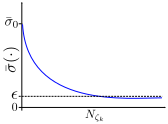
\includegraphics[width=0.95\columnwidth]{fig/knowledge_idealization.png}
	\caption{Remaining knowledge to learn a new skill $s_{j,k}$.}
	\label{fig:knowledge_idealization}
\end{figure}
% ---
% ===================================================================================================
\subsection{Knowledge sharing and transfer under different learning paradigms}
%The following assumptions are analogous to average behavior and imply that a suitable scaling strategy is available and executed.
%Before tacking the different learning schemes let us define the idealized reference system in which a large number of robots coexists learning a large number of skills.

For the upcoming analysis we consider an idealized reference system in which a large number of robots coexist learning a large number of skills. Such system exhibits
% ---
\begin{tcolorbox}
	\begin{assumption}\label{assumption:average_behavior}
		An average behavior that results from comparable EAI agents learning and executing the skills in $\mathcal{S}$ ordered and segregated according to their similarity.
	\end{assumption}
\end{tcolorbox}
%---
Each of the EAI agents in the system
\begin{tcolorbox}
	\begin{assumption}\label{assumption:agent_similarity}
		Has the same capabilities with highly similar BEE and MIE expenditures.
	\end{assumption}
\end{tcolorbox}
%---
The large number of skills in $\mathcal{S}$ implies that
% ---
\begin{tcolorbox}
	\begin{assumption}\label{assumption:cluster_size}
		Every cluster $\mathcal{Z}_{k}$ contains the same number $N_{\mathcal{Z}} $ of skills.
	\end{assumption}
\end{tcolorbox}
% ---
By virtue of the optimal ordering of the skills and the balanced size of the clusters,
% ---
\begin{tcolorbox}
	\begin{assumption}\label{assumption:cluster_transferability}
		The knowledge transferability between in-cluster skills ---modeled by \eqref{eq:f_function_incremental} and \eqref{eq:g_function_incremental}--- is assumed to be equal; as is transferability between clusters, see \eqref{eq:f_function_transfer} and \eqref{eq:g_function_transfer}.
	\end{assumption}
\end{tcolorbox}
% ---
Finally, the different learning paradigms that exploit the collected knowledge by the EAI agents rely on the fact that
% ---
\begin{tcolorbox}
	\begin{assumption}\label{assumption:enabling_agorithms}
	There are advanced control and machine learning algorithms designed to inherently use this knowledge.
	\end{assumption}
\end{tcolorbox}

% ---------------------------------------------------------------------------------------------------
\subsubsection{\textbf{Isolated Learning (IsL)}} A robot learns each skill in $\mathcal{Z}_k$ one after another from the ground up, disregarding the accumulating knowledge from already learned skills. In such a case the rate of convergence and the initial remaining knowledge for all skills are given by
% ---		
\begin{subequations}\label{eq:fg_isolated}
	\begin{alignat}{2}
		f_{j,k}\left(\cdot \right) &=  -\alpha \\
		g_{j,k}\left(\cdot \right) &= 1,
	\end{alignat}
\end{subequations}
% ---
where $ \alpha>0$ models the rate at which a robot in isolation learns any given skill. Relying on Asm.~\ref{assumption:agent_similarity} we can assign a value to $\alpha$ by using the fundamental complexity $c_0$ as follows
% ---
\begin{equation}\label{eq:isolated_learning_rate}
	\alpha = -\frac{1}{c_0}\text{log}(\epsilon).
\end{equation}
% ---
Since in isolated learning $c^{(IsL)}_{j,k} = c_0$, the trial episodes required by one single robot to learn the skills in the cluster $\mathcal{Z}_k$ is given by
% ---
\begin{align}
	\begin{split}
		C^{(IsL)}_{k} &= \sum_{j=1}^{N_{\mathcal{Z}}} c^{(IsL)}_{j,k}= N_{\mathcal{Z}}  \cancelto{c_{0}}{c^{(IsL)}_{j,k}} = N_{\mathcal{Z}} c_0
	\end{split}
\end{align}
%-- 
Similarly, the total trial episodes to learn the universe of skills is simply
% ---
\begin{equation}
	C^{(IsL)}_{\mathcal{S}} = N_\mathcal{K} N_{\mathcal{Z}} c_0.
\end{equation}
% ---
\paragraph*{Multi agent case}
Suppose that a batch of $m$ robots is used to learn the same number of skills in parallel in a given cluster $\mathcal{Z}_k$. Such a strategy only distributes equally the total number of episodes by the number of available robots; i.e.
% ---
\begin{equation}
	^{\lvert \lvert}C^{(IsL)}_k=  \overbrace{\frac{1}{m}C^{(IsL)}_k}^{\text{episodes per robot}}.
\end{equation}
% ---




%The energy required by one single robot to learn the skills in the cluster $\mathcal{Z}_k$ is given by
%% ---
% \begin{align}
%     \begin{split}
%       E^{(Iso)}_{\mathcal{Z}_k} &= \sum_{j=1}^{N_{\mathcal{Z}}} E^{(Iso)}_j= N_{\mathcal{Z}_k}  e_{0} \cancelto{c_{0}}{c_{j,k}} = N_{\mathcal{Z}} e_{0}  c_0
%     \end{split}
% \end{align}
%%-- 
%If $\mathcal{S}$ is divided into $\left\lbrace \mathcal{Z}_k \right\rbrace^{N_\mathcal{K}}_{k=1} $ clusters, the total energy to learn the universe of skills is simply
%% ---
%\begin{equation}
%	E^{(Iso)}_{\mathcal{S}} = N_\mathcal{K} N_{\mathcal{Z}} e_{0}  c_0.
%\end{equation}
%% ---
%\paragraph*{Multi agent case}
%Notice that using a batch of $m$ robots to learn the same number of skills in parallel does not bring about any energy reductions since
%% ---
%\begin{equation}
%    ^{\lvert \lvert}E^{(Iso)}_\mathcal{S}= \underbrace{m}_{\text{robots}}\cdot \overbrace{\frac{1}{m}E^{(Iso)}_\mathcal{S}}^{\text{energy per robot}} = E^{(Iso)}_\mathcal{S}.
%\end{equation}
%% ---


%---
% \begin{figure}[!ht]
% 	\centering
% 	\includegraphics[width=0.99\columnwidth]{tex/fig/single_incremental_knowledge.pdf}
% 	\caption{Knowledge sharing in incremental learning. A single agent leverages previously acquired knowledge from other learned skills in $\mathcal{Z}$.}
% 	\label{fig:single_incremental_knowledge}
% \end{figure}

% ---
\begin{figure}[!t]
	\centering
	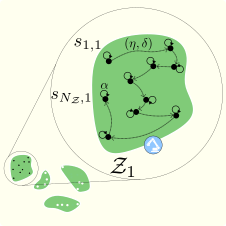
\includegraphics[width=0.95\columnwidth]{fig/intra_skill_learning.png}
	\caption{Incremental learning benefits from the significant similarity of skills belonging to the same cluster.}
	\label{fig:intra_skill_learning}
\end{figure}
% ---
% ---
\begin{figure*}[!htb]
	\centering
	\hspace*{\fill}
	\subfloat[]{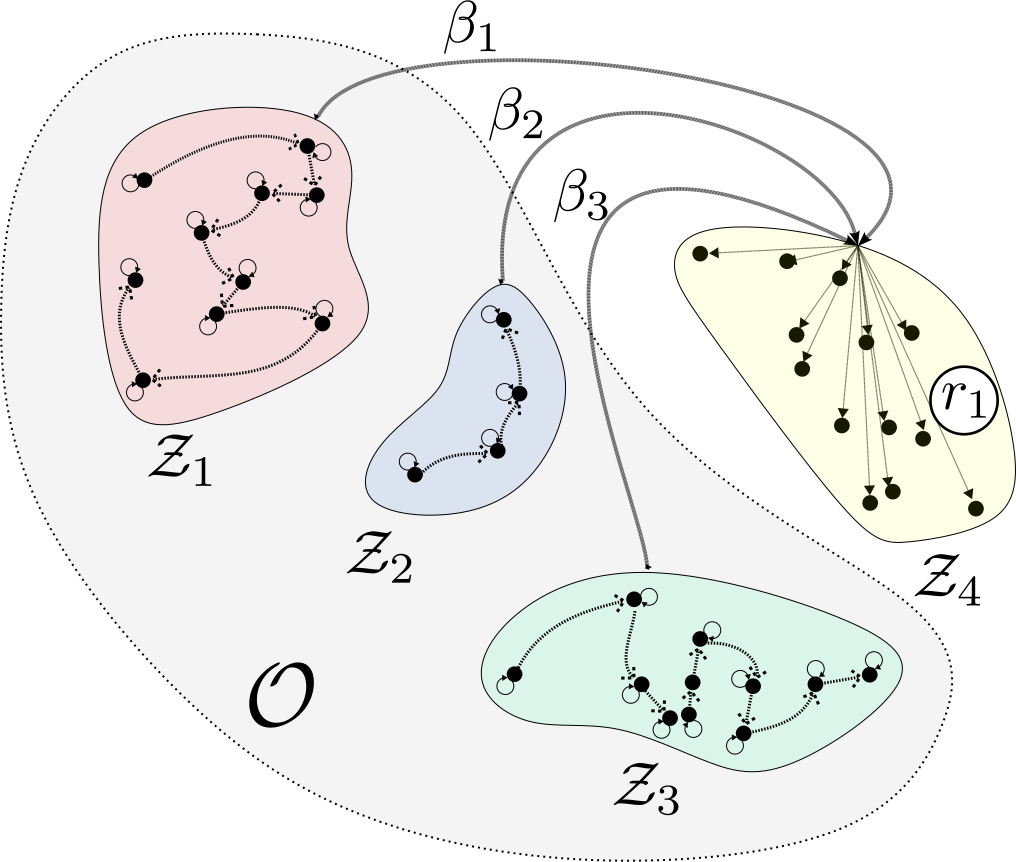
\includegraphics[width= 0.45\textwidth]{fig/cluster_to_cluster_knowledge_transfer.png} \label{fig:cluster_to_cluster_knowledge_transfer}}  
	\hfill	
	\subfloat[]{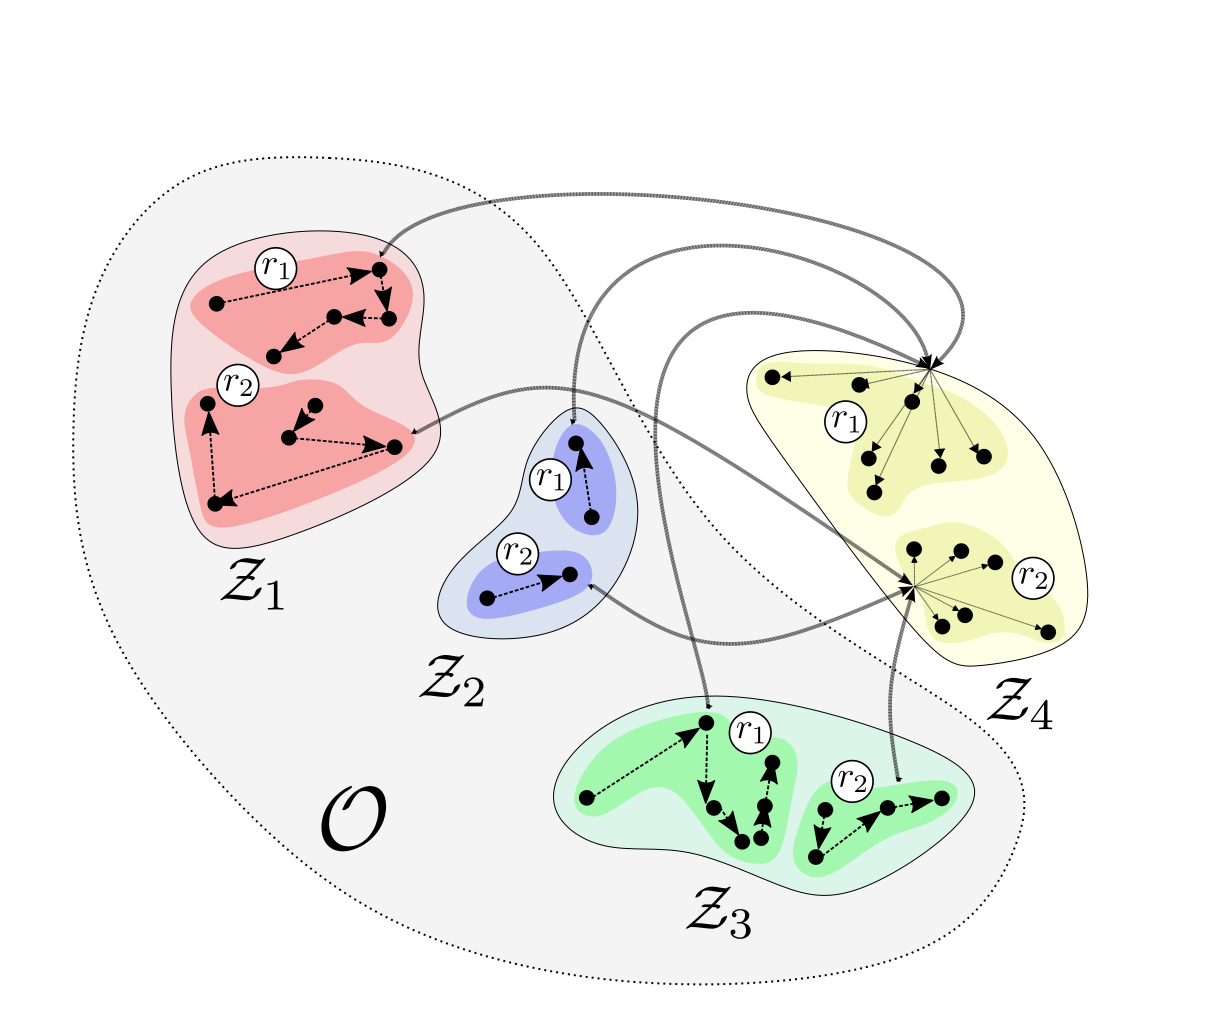
\includegraphics[width= 0.45\textwidth]{fig/cluster_to_cluster_knowledge_transfer_parallel.png} \label{fig:cluster_to_cluster_knowledge_transfer_parallel}}
	\hspace*{\fill}
	\caption[] {\label{fig:tranfer_learninhg} Transfer learning. \subref{fig:cluster_to_cluster_knowledge_transfer} Transfer of knowledge from different origin clusters to the target cluster,  \subref{fig:cluster_to_cluster_knowledge_transfer_parallel} using many robots (e.g. two robots $r_1$ and $r_2$) without knowledge exchange among them only subdivides the problem.}
\end{figure*}
% ---
% ---------------------------------------------------------------------------------------------------
\subsubsection{\textbf{Incremental Learning (IL)}}
It corresponds to the continuous aggregation and exchange of knowledge from \emph{intra-cluster} skills. Referring back to Asm.~\ref{assumption:skill_clustering}, the knowledge from skills belonging to a cluster ${\mathcal{Z}_k}$ can be be leveraged by an agent in virtue of their significant similarity. As depicted in Fig.~\ref{fig:intra_skill_learning}, a robot ($r_1$ in this case) learns every skill in $\mathcal{Z}_1$ with a rate $\alpha$ ---the self loops--- but also retains and uses the acquired knowledge to learn subsequent skills. The effect of incremental learning on the knowledge collection rate can be modeled to be directly proportional to the number of learned skills as
% ---
\begin{equation}\label{eq:f_function_incremental}
	f_{j,k}\left(N_{\zeta_k}\right) = -\alpha\left(\eta N_{\zeta_k} + 1 \right), 
\end{equation}
% ---
where $\eta>0$ represents the efficiency of knowledge exchange from $\zeta_k$ to $s_{j,k}$. Different potential models might be used to model the depletion of the initial remaining knowledge represented by $g_{j,k}\left(N_{\zeta_k}\right)$, e.g. a linear decay rate, our expectation is that, under the assumption that a learning strategy involving the ordering of skills according to similarity and their balanced distribution in the different clusters, $g_{j,k}\left(N_{\zeta_k}\right)$ might naturally resemble an exponential decay that is strongly dependent on $N_{\zeta_k}$. Such considerations motivate our choice of the following function
% ---
\begin{equation}\label{eq:g_function_incremental}
	g_{j,k}\left(N_{\zeta_k}\right) = e^{-\delta N_{\zeta_k}},
\end{equation}
%---
again with a factor $\delta>0$ controlling the rate at which the exponential converges. Similar to $\alpha$, using Asm.~\ref{assumption:cluster_size} $\delta$ can be defined as 
% ---
\begin{equation}\label{eq:delta}
	\delta = -\frac{1}{N_\mathcal{Z}}\text{log}(\epsilon).
\end{equation}
% ---
Essentially, such choice of $\delta$ implies that the remaining knowledge in a cluster after seeing all its skills is negligible. Via the exchange factors $(\eta,\delta)$, in incremental learning the knowledge about every new skill gets gradually increased by leveraging previous knowledge, resulting in
% ---
\begin{equation*}\label{eq:remaining_knowledge__IL}
	\bar{\sigma}^{(IL)}_{i,j}(n) = e^{-\alpha  \left(\eta N_{\zeta_k}+1\right) n} e^{-\delta N_{\zeta_k}}.
\end{equation*}
% ---
As the complexity $c_{j,k}$ of a skill can also be interpreted as the number of trial episodes required for the remaining knowledge to go below a threshold $\epsilon$; i.e.
% ---
\begin{equation*}
	\bar{\sigma}^{(IL)}_{i,j}(n) \Big \rvert_{n \ge c^{(IL)}_{j,k}} \leq \epsilon.
\end{equation*}
% ---
Then, under this scheme the complexity $c^{(IL)}_{j,k}$ to learn a new is skill in the cluster results in
%\begin{equation}\label{eq:complexity_IL}
%	c^{(I)}_{j,k} = -\frac{\text{log}(\epsilon)}{\alpha \eta (N_{\zeta_k}+ 1)}.
%\end{equation}
\begin{equation}\label{eq:complexity_IL}
	c^{(IL)}_{j,k} = -\frac{\text{log}(\epsilon) - \text{log}\left(\bar{\sigma}^{(IL)}_{j,k}(0)\right)}{\alpha (\eta N_{\zeta_k}+ 1)} = -\frac{\text{log}(\epsilon) + \delta N_{\zeta_k}}{\alpha (\eta N_{\zeta_k}+ 1)}  .
\end{equation}
% ---
The total number of trial episodes $ C_k $ that an agent following an incremental learning strategy needs to learn the $N_{\mathcal{Z}_k}$ skills in a cluster $ \mathcal{Z}_k $ is given by
% ---
\begin{align}\label{eq:total_episodes_incremental}
	\begin{split}
		C^{(IL)}_k &= \sum^{N_{\mathcal{Z}}}_{j=1} c^{(IL)}_{j,k}.
	\end{split}
\end{align}
% ---

\paragraph*{Multi-agent case}
If $m$ robots are used in parallel to divide the load of learning the tasks then
% ---
\begin{align}
	\begin{split}
		{}^{\lvert \rvert}C^{(IL)}_k &= \sum^{\frac{N_{\mathcal{Z}}}{m}}_{j=1} c^{(IL)}_{j,k}.
	\end{split}
\end{align}
% --
In essence, using $m$ robots without exchanging knowledge only subdivides the learning in every cluster into $m$ smaller problems \emph{without adding any additional benefit to the rate at which knowledge is acquired}. 

\subsubsection{\textbf{Transfer + Incremental Learning (TIL)}}
Transfer learning (TL) alone refers to the one-time \emph{inter-cluster} exchange of knowledge. Considering $\mathcal{K} = \{ \mathcal{Z}_k \}^{N_\mathcal{K}}_{k=1}$ to be the set of all available skill clusters, TL represents the exchange of knowledge from the skills learned in different \emph{origin} clusters $\mathcal{O} = \{ \mathcal{Z}_1,\mathcal{Z}_2,\ldots,\mathcal{Z}_{k-1} \}$ to the skills that will be learned in a \emph{destination} cluster $\mathcal{Z}_k$ (see Fig.~\ref{fig:cluster_to_cluster_knowledge_transfer}). Concretely, the effect that TL has on the skills of the destination cluster is the reduction of the initial remaining knowledge and the increase of the initial learning rate for all the skills in the $k$-th cluster via the parameter $\beta_k$; i.e.
% ---
\begin{equation}\label{eq:f_function_transfer}
	f_{j,k}\left(N_{\zeta_k}\right) = -\alpha \left( \frac{\eta N_{\zeta_k} + 1}{1 - \beta_k} \right),
\end{equation}
% ---
and
% ---
\begin{equation}\label{eq:g_function_transfer}
	g_{j,k}\left(N_{\zeta_k}\right) = (1-\beta_k) e^{-\delta N_{\zeta_k}}.
\end{equation}
%---
In essence, $\beta_k$ is the head start granted by knowledge transfer from other clusters to the skills in $\mathcal{Z}_k$. We argue that  $0<\beta_{k} < 1$ since it represents the \emph{aggregated} knowledge exchange factor from the different origin clusters $\mathcal{Z}_{c}$ to the target cluster $\mathcal{Z}_{k}$. Let $0<\beta_{c} < 1$ be the transfer contribution factor of a single origin cluster $\mathcal{Z}_c$. Additionally, consider that
% ---
\begin{equation}
	\sum\limits_{c=1}^{N_\mathcal{K}}\beta_{c} \leq 1,
\end{equation}
% --
as $1$ represents all the knowledge in $\mathcal{S}$. Asm.~\ref{assumption:cluster_transferability} implies that $\beta_c$ is equal for all the clusters. In this work we select $\beta_c = 1/N_\mathcal{K}$ for simplicity. The aggregated transfer factor $\beta_k$ is the sum of the individual factors from the already-visited clusters; i.e.
% ---
\begin{equation}\label{eq:beta_k_transfer}
	\beta_{k}= \left(k-1\right)\beta_c = \left(k-1\right)\frac{1}{N_\mathcal{K}}.
\end{equation}
% ---

Consequently, the remaining knowledge when transfer and incremental learning are used in conjunction is
% ---
\begin{equation}\label{eq:remaining_knowledge__ITL}
	\bar{\sigma}^{(TIL)}_{j,k}(n) = \left(1- \beta_k\right) e^{-\alpha  \left(\frac{ \eta N_{\zeta_k}+1}{1 - \beta_k}\right) n} e^{-\delta N_{\zeta_k}}.
\end{equation}
% ---
Similar to incremental learning, the complexity to learn a skill in transfer learning is
\begin{equation}\label{eq:skill_complexity_TL}
	c^{(TIL)}_{j,k} = -\frac{1 - \beta_{k}}{\alpha (\eta N_{\zeta_k}+ 1)}\left[\text{log}(\epsilon) + \delta N_{\zeta_k} - \text{log}(1 - \beta_{k})\right]
\end{equation}
% ---
and the total number of episodes  $ C_k $ that an agent requires to learn the $N_{\mathcal{Z}_k}$ skills is merely their sum
% ---
\begin{align}\label{eq:total_episodes_transfer}
	\begin{split}
		C^{(TIL)}_k &= \sum^{N_{\mathcal{Z}}}_{j=1} c^{(TIL)}_{j,k}.
	\end{split}
\end{align}
% --- 

\paragraph*{Multi-agent case}
If $m$ robots are used in parallel to divide the load of learning the tasks then, the transfer of knowledge from cluster to cluster is also divided by the number of robots, this implies that \eqref{eq:beta_k_transfer} changes to
% ---
\begin{equation}\label{eq:beta_k_transfer_parallel}
	{}^{\lvert \rvert}\beta_{k}= \frac{1}{m}\beta_{k}.
\end{equation}
% ---
Correspondingly, when using transfer learning in parallel $\beta_k$ is replaced by ${}^{\lvert \rvert}\beta_{k}$ in \eqref{eq:skill_complexity_TL}. Then, similar to IL, the total number of episodes to learn the skills in a cluster is
% ---
\begin{align}
	\begin{split}
		{}^{\lvert \rvert}C^{(TIL)}_k &= \sum^{\frac{N_{\mathcal{Z}}}{m}}_{j=1} c^{(TIL)}_{j,k}.
	\end{split}
\end{align}
% ---
This case is depicted on Fig.~\ref{fig:cluster_to_cluster_knowledge_transfer_parallel}, where two robots $ r_1$ and $r_2$ learn skills in four different clusters. The shaded areas are the subclusters of skills learned by each robot. Since they do not share knowledge between them, each robot has access only to the knowledge it has collected and cannot benefit from one another. 

% ---------------------------------------------------------------------------------------------------
\subsubsection{\textbf{Collective learning (CL)}}
As mentioned in Sec.~\ref{sec:intro}, EAI agents will be a core element of industrial, healthcare, and domestic ecosystems with advanced communication and remote processing capabilities. Given the anticipated legions of EAI agents executing and learning several different skills at any given time in those environments, it is immediately evident that the previous learning paradigms are not meant to exploit these large number of agents together with the advanced communication and processing infrastructure to take full advantage of the potential for concurrent knowledge exchange among the agents. Therefore, the use of isolated, incremental, and transfer learning by these many agents 
would directly aggravate computational demand (see \textbf{challenge 1} in Sec.~\ref{sec:robots_challenge}). As discussed in \cite{Kaelbling2020foundationefficientrobot} an leaning algorithm that would allow an agent to learn new tasks on-the-fly would need to be sample-efficient, generalizable, compositional, and (truly) incremental. Collective learning is the natural paradigm that meets this requirements exploiting the full communication potential of the networked EAI agents to leverage the real-time synergistic exchange and aggregation of collected knowledge to make the learning of tasks energy- and time-efficient.

To formalize this idea, let $ \left\lbrace \rho_i \right\rbrace_{i=1}^{m} $ be a set of robotic agents that defines a community of robots. In collective learning, the different robotic agents $ \rho_i $ develop and accumulate dynamically a common mind (body of knowledge) via networked interactions where individual experience, knowledge and skills are disseminated to all the other elements in the collective. Information flows vertically as previous knowledge is passed on, as well as horizontally by sharing concurrent experience between agents. Via these mechanisms, knowledge can be replicated, complimented and further developed. We take from \cite{Garavan2012CollectiveLearning} two notions central in collective learning that are applicable to the embodied AI agents:
% ---
\begin{enumerate}
	\item Capability to restructure and meet changing conditions
	\item Aggregation of skills, knowledge, and behaviors
\end{enumerate}
% ---
Collective learning contrasts with the previously discussed incremental learning in that a single agent $ r_i $ can aggregate only so much knowledge via trial and error and is limited by a sequential learning structure. Learning collectively, on the other hand, enforces parallelization of knowledge acquisition via the concurrent learning and sharing of all agents as they acquire new skills, knowledge. Moreover, collective learning involves not only the information acquisition, but also how this information is brought to use to form and develop knowledge. 

CL is not only a promising research direction but, in our opinion, has the potential to be a unifying solution to the grand challenges posed by embodied AI. Furthermore, by incorporating new mechanical designs as elements of the learning pipeline it is possible to iteratively evaluate the energy efficiency of proposed solutions and select the best ones as reference designs for future manufacturing processes with underlying learning, therefore, promoting a cyclical optimization towards a semi-optimal general design.
% ---
\begin{figure}[!th]
	\centering
	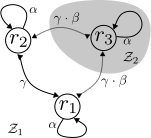
\includegraphics[width=0.7\columnwidth]{fig/cl_example_figure.png}
	\caption{Exchange of knowledge between EAI agents enables collective learning.}
	\label{fig:cl_example_figure}
\end{figure}
% ---

Unlike isolated and transfer learning, in this paradigm a batch of robots $\left \lbrace r_i \right \rbrace^m_{1}$ not only learn different skills concurrently but also exchange the acquired knowledge between each other and are actually able to leverage it. To enable CL, it is assumed that
\begin{itemize}
	\item an inter-agent communication protocol/infrastructure is in place that
	\item enables agents to concurrently exchange and integrate the self-acquired and received knowledge to
	\item incrementally speed up the learning of all the agents as a whole.
\end{itemize}
% ---
As a result, the intra- and inter-cluster knowledge transfer is possible. Naturally, the CL paradigm involves a complex scheduling problem to determine the optimal skill distribution and inter-agent knowledge sharing strategy. Since we have not tackled this problem yet, we ground the subsequent discussion on Assumptions~\ref{assumption:average_behavior}, \ref{assumption:agent_similarity},~\ref{assumption:cluster_size}, and~\ref{assumption:cluster_transferability} that suggest an average behavior given a suitable scheduling.

Fig.~\ref{fig:cl_example_figure} illustrates the CL concept, where the self loop represents the dynamics of a single robot learning (at a rate $\alpha$). The exchange of knowledge across agents is represented via the cross-couplings weighted by a parameter $\gamma$ that models how efficient is the bidirectional pairwise knowledge exchange. Similar to transfer learning, if two robots exchange knowledge about skills with low similarity (i.e. skills in different clusters), then $\gamma$ is scaled by the inter-cluster transferability parameter $\beta$. In CL \eqref{eq:simple_knowledge_dynamics} is extended to 
% ---
\begin{subequations}\label{eq:collective_knowledge_dynamics}
	\begin{alignat}{2}
		\dot{\bar{\bm{\sigma}}}^{(CL)}_{j,k}\left(n\right) &= \overbrace{\left[  f_{j,k}\left(N_{\zeta_k},r\right) \bm{I} + \gamma \bm{A} \odot \bm{B}  \right]}^{\bar{\bm{A}}\left(N_{\zeta_k}\right)} \bar{\bm{\sigma}}^{(CL)}_{j,k}\left(n\right)\\
		\bar{\bm{\sigma}}^{(CL)}_{j,k}(0) &= g_{j,k}\left( N_{\zeta_k}, r\right) \bm{I},
	\end{alignat}
\end{subequations}
% ---
where $r=m$ is the number of robots that exchange knowledge among them. This implies that now $\bar{\bm{\sigma}}^{}_{j,k} \in \mathbb{R}^r$ is a vector that represents the dynamics of the remaining knowledge of all the $m$ skills being concurrently learned. $\bm{A} \in \mathbb{R}^{r \times r}$ is a zero-diagonal symmetric adjacency matrix whose entry $(\bm{A})_{i,j} = 1$ if robot $i$ exchanges knowledge with robot $j$ and $(\bm{A})_{i,j} = 0$ if it does not. The term $\gamma \in \mathbb{R}_+ $ weighs the knowledge exchange strength among robots. Furthermore, since there may be robots learning skills in different clusters at the same time, the matrix $\bm{B}$, whose entries are $\left(\bm{B}\right)_{i,j} \in \left \lbrace 1, \beta_{k} \right \rbrace$, with
% ---
\begin{equation}
	%\beta_{k} = 1/N_\mathcal{K}, 
	\beta_{k} = r\frac{ N_{\zeta_k}}{N_\mathcal{S}}, 
\end{equation}
% ---
scales down the knowledge contributions between robots from different clusters. Finally, the operator $\odot$ represents the Hadamard product of matrices. The functions $ f(\cdot)$ and $g(\cdot)$ are now also dependent on the number of robots that exchange knowledge, which directly impacts the number of skills that enter $\zeta_k$ after a learning cycle; i.e.
% ---
\begin{equation}\label{eq:f_function_collective}
	f_{j,k}\left(N_{\zeta_k},r\right) = -\alpha \left( \frac{\eta r N_{\zeta_k} + 1}{1 - \beta_k} \right),
\end{equation}
% ---
and
% ---
\begin{equation}\label{eq:g_function_collective}
	g_{j,k}\left(N_{\zeta_k},r\right) = (1-\beta_k) e^{-\delta r N_{\zeta_k}}.
\end{equation}
%---
Some considerations need to be taken when selecting the value of $\gamma$ given that the dynamics matrix of the collective system
% ---
\begin{equation}
	\bar{\bm{A}}\left(N_{\zeta_k}\right) = f\left(N_{\zeta_k},r\right) \bm{I} + \gamma \bm{A} \odot \bm{B} 
\end{equation} 
% ---
exhibits a dependency on the number of seen skills $N_{\zeta_k}$, which is directly influenced by the number of robots $r$ in the collective. Yet, it can be proven that there is a coupling strength $\gamma$ for a given connectivity $\bm{A}$ that ensures that the remaining knowledge for all skills converges asymptotically to zero.

\TODO \textcolor{red}{is there an approximation of the convergence rate of all the skills?}




